\enquestion{8.29}{
    A postmix beverage machine is adjusted to release a certain amount of syrup into a chamber where it is mixed with carbonated water.
    A random sample of $25$ beverages was found to have a mean syrup content of $\bar{x} = 30\text{ mL}$ and a standard deviation of $s = 0.5\text{ mL}$.
    Find a \SI{95}{\percent} CI on the mean volume of syrup dispensed.
}
\enanswer{
    $[29.7936, 30.2064]$
}

\enquestion{8.37}{
    The compressive strength of concrete is being tested by a civil engineer who tests $10$ specimens and obtains the following data:
    
    \begin{center}
        \begin{tabular}{*{4}{C{0.225\textwidth}}}
            $2216$ & $2237$ & $2249$ & $2204$ \\
            $2225$ & $2301$ & $2281$ & $2263$ \\
            $2318$ & $2255$ & &
        \end{tabular}
    \end{center}
    
    \begin{enumerate}[label=(\alph*)]
        \item Check the assumption that compressive strength is normally distributed.
        Include a graphical display in your answer.
        \item Construct a \SI{95}{\percent} two-sided confidence interval on the mean strength.
        \item Construct a \SI{95}{\percent} lower confidence bound on the mean strength.
        Compare this bound with the lower bound of the two-sided confidence interval and discuss why they are different.
    \end{enumerate}
}
\enanswer{
    \begin{enumerate}[label=(\alph*)]
        \item Normal probability plot:
        \begin{center}
            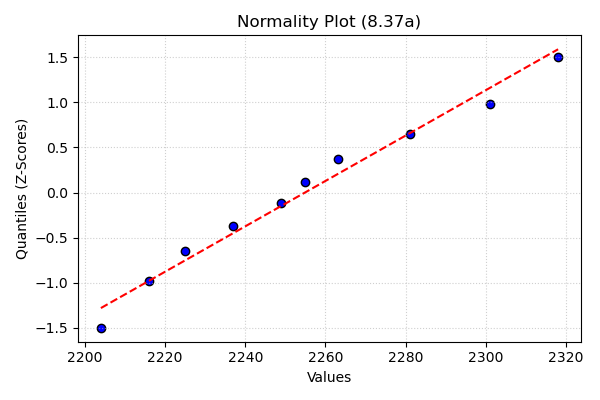
\includegraphics[scale=0.7]{../../figures/opg8.37a.png}
        \end{center}
        The points lie reasonably close to a straight line, indicating that the compressive strength data can be assumed to be normally distributed.
        \item $[2228.5565, 2281.2435]$
        \item $[2233.5527, \infty)$
    \end{enumerate}
}

\enquestion{8.39}{
    An article in \textit{Computers \& Electrical Engineering} [\enquote{Parallel Simulation of Cellular Neural Networks} (1996, Vol. 22, pp. 61--84)] considered the speedup of cellular neural networks (CNN) for a parallel general-purpose computing architecture based on six transputers in different areas.
    The data follow:

    \begin{center}
        \begin{tabular}{*{5}{C{0.17\textwidth}}}
            $3.775302$ & $3.350679$ & $4.217981$ & $4.030324$ & $4.639692$ \\
            $4.139665$ & $4.395575$ & $4.824257$ & $4.268119$ & $4.584193$ \\
            $4.930027$ & $4.315973$ & $4.600101$ & &
        \end{tabular}
    \end{center}

    \begin{enumerate}[label=(\alph*)]
        \item Is there evidence to support the assumption that speedup of CNN is normally distributed?
        Include a graphical display in your answer.
        \item Construct a \SI{95}{\percent} two-sided confidence interval on the mean speedup.
        \item Construct a \SI{95}{\percent} lower confidence bound on the mean speedup.
    \end{enumerate}
}
\enanswer{
    \begin{enumerate}[label=(\alph*)]
        \item Normal probability plot:
        \begin{center}
            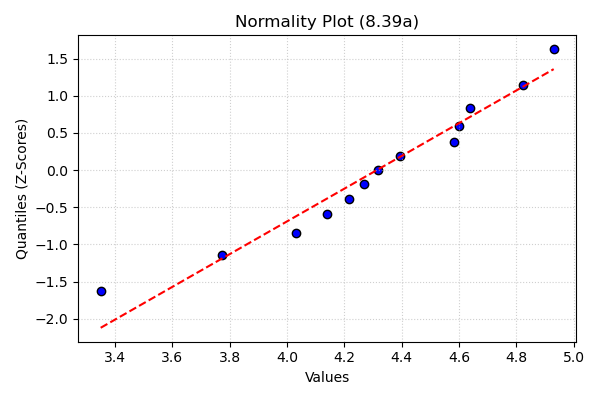
\includegraphics[scale=0.7]{../../figures/opg8.39a.png}
        \end{center}
        The points approximate a straight line, showing that the speedup is normally distributed.

        \item $[4.0517, 4.5748]$
        \item $[4.0993, \infty)$
    \end{enumerate}
}

\enquestion{8.41}{
    An article in \textit{Nuclear Engineering International} (February 1988, p.~33) describes several characteristics of fuel rods used in a reactor owned by an electric utility in Norway.
    Measurements on the percentage of enrichment of $12$ rods were reported as follows:
    \begin{center}
        \begin{tabular}{*{6}{C{0.14\textwidth}}}
            $2.94$ & $3.00$ & $2.90$ & $2.75$ & $3.00$ & $2.95$ \\
            $2.90$ & $2.75$ & $2.95$ & $2.82$ & $2.81$ & $3.05$
        \end{tabular}
    \end{center}
    \begin{enumerate}[label=(\alph*)]
        \item Use a normal probability plot to check the normality assumption.
        \item Find a \SI{99}{\percent} two-sided confidence interval on the mean percentage of enrichment.
        Are you comfortable with the statement that the mean percentage of enrichment is $2.95\%$?
        Why?
    \end{enumerate}
}
\enanswer{
    \begin{enumerate}[label=(\alph*)]
        \item The data appear to be normally distributed.
        \item $[2.8126, 2.9907]$, yes, because $2.95 \in \text{CI}$.
    \end{enumerate}
}